\clearpage
\section{Additional Plots}
\label{app:plots}

\subsection{Taka Detector Precision--Recall Curve}
\begin{figure}[H]
  \centering
  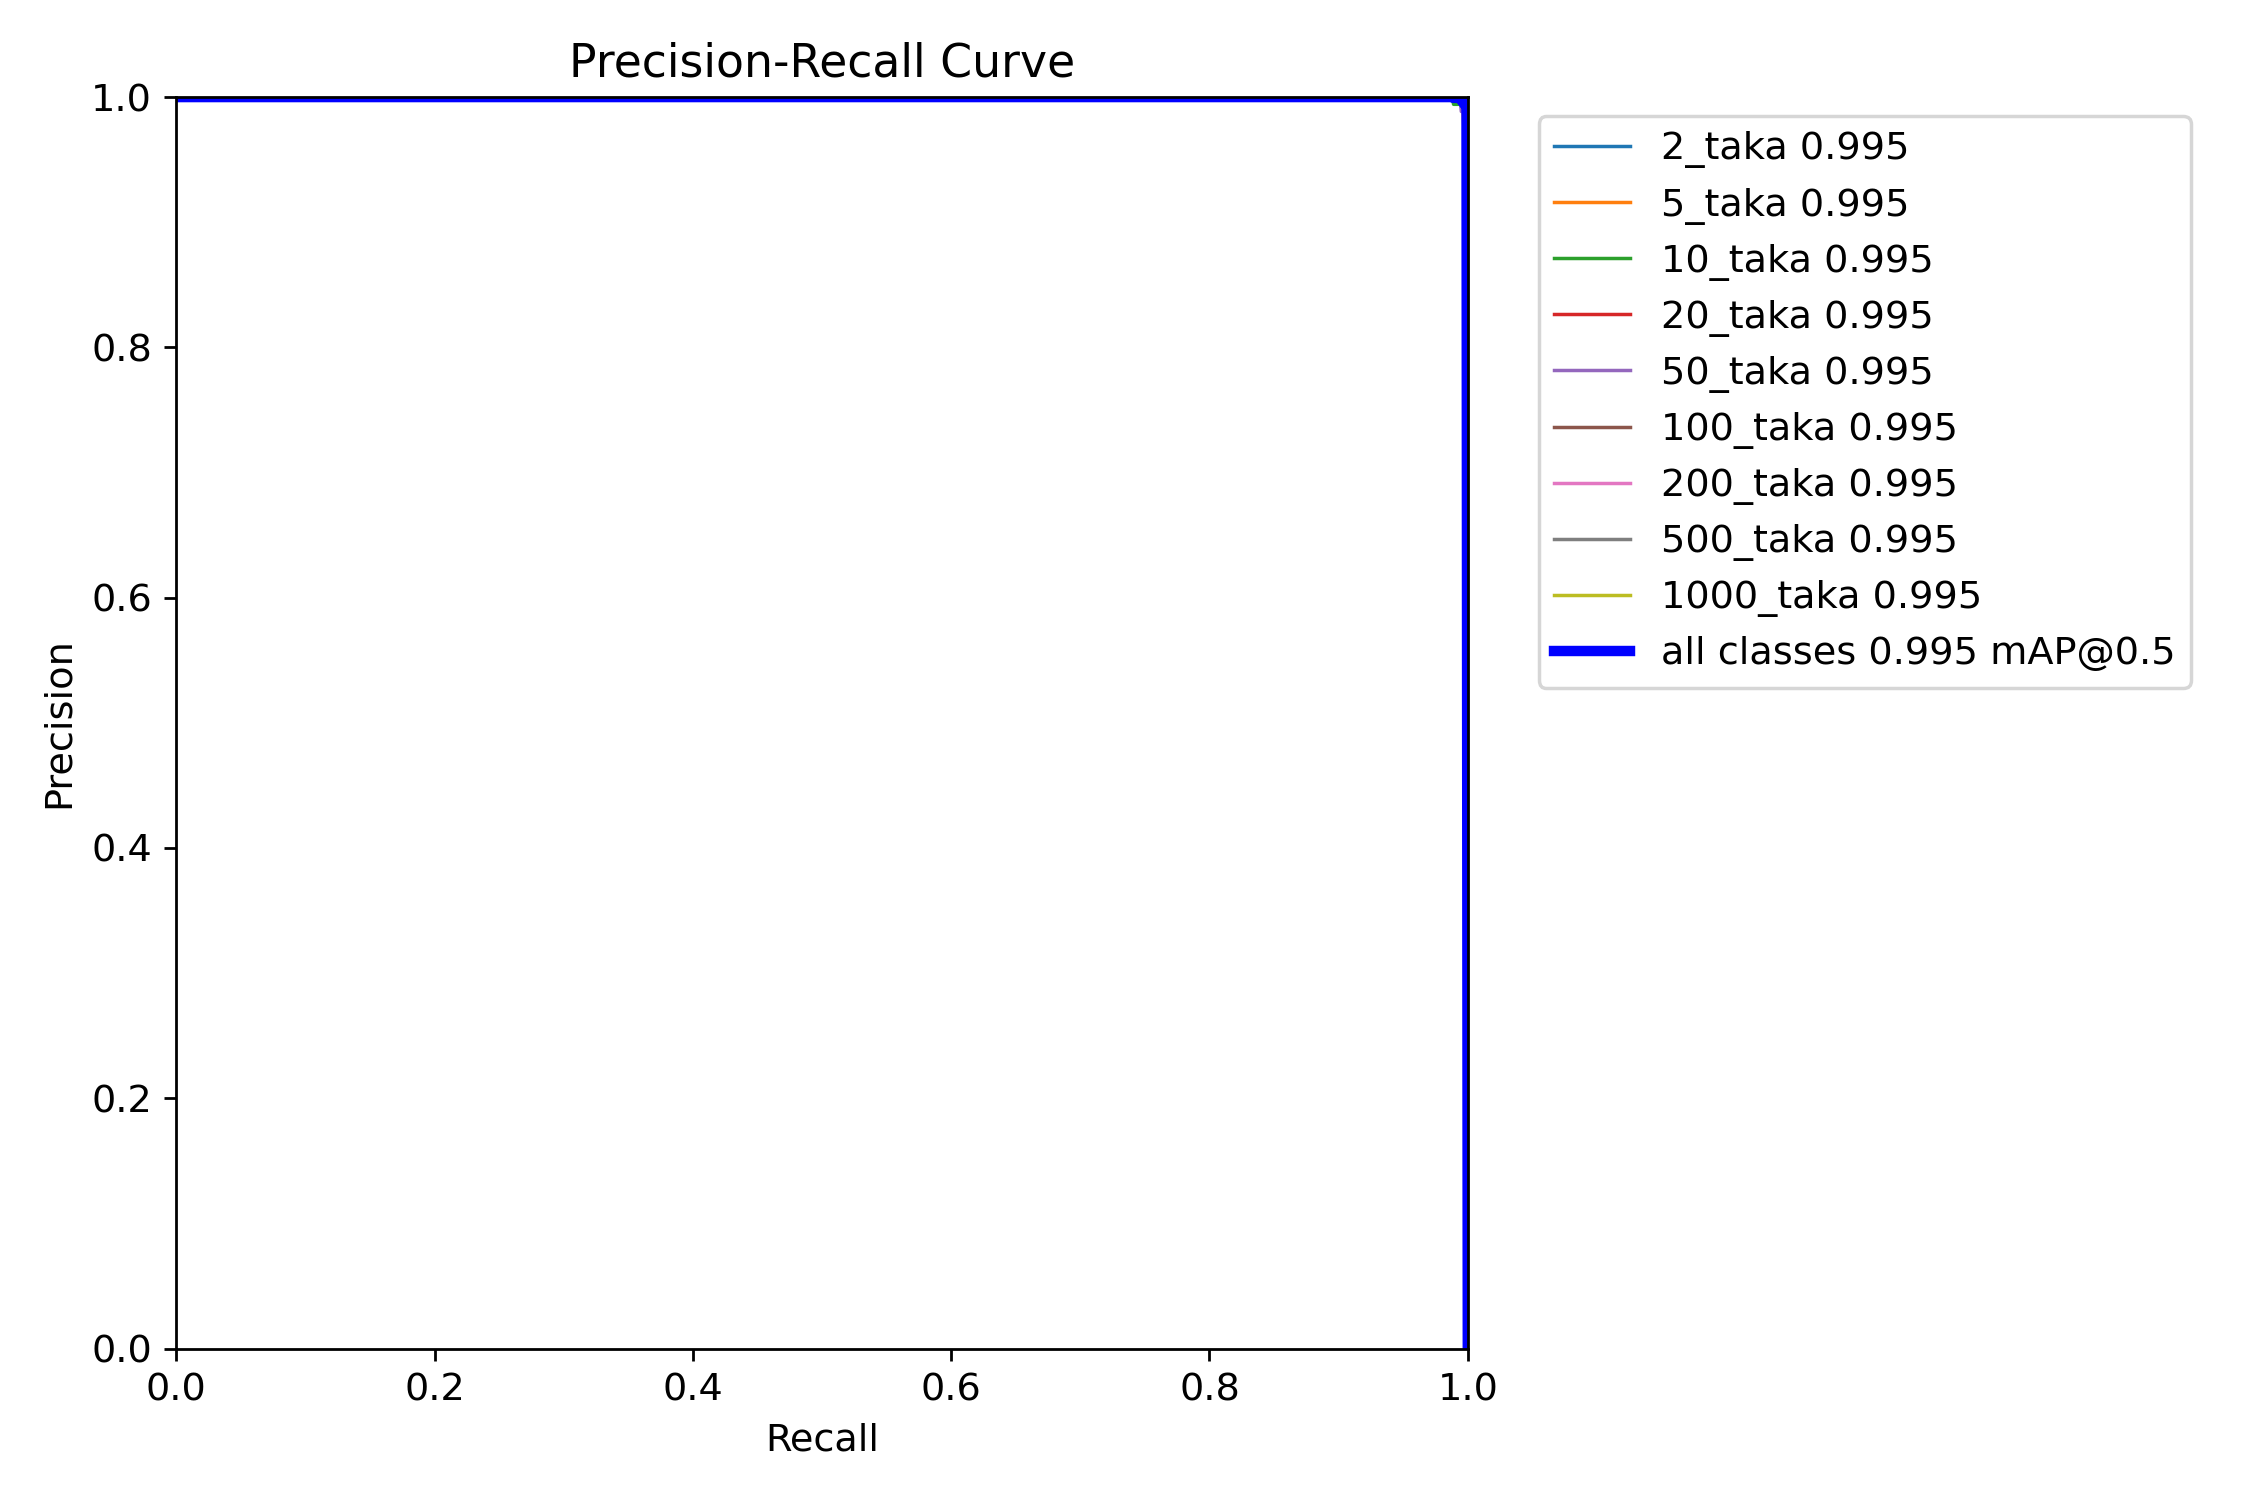
\includegraphics[width=0.75\textwidth]{fig_pr_curve.png}
  \caption{Precision--recall curves of the YOLOv8s Taka detector for all nine classes on the held-out synthetic test set}
  \label{fig:app_pr}
\end{figure}

\subsection{Sample Detections}
\begin{figure}[H]
  \centering
  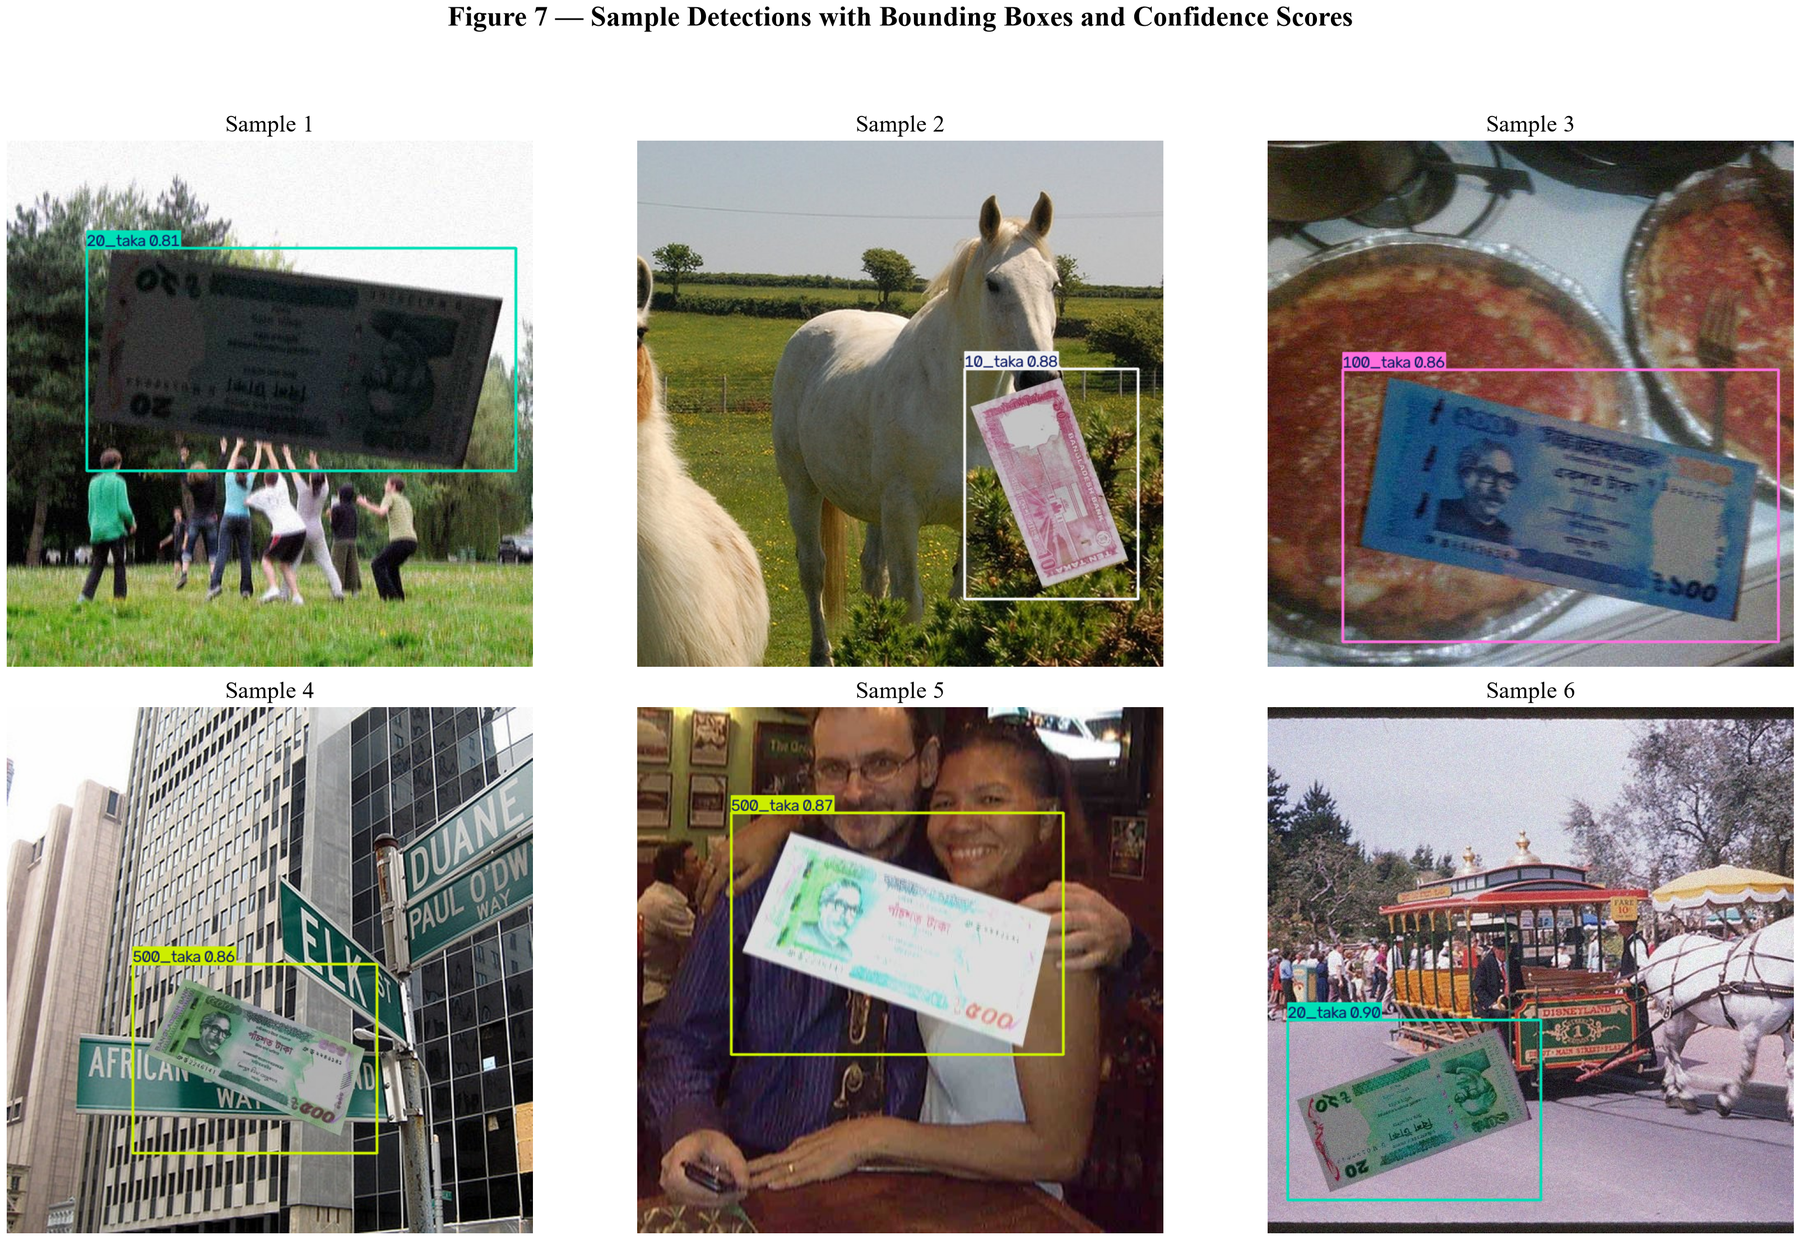
\includegraphics[width=\textwidth]{fig7_sample_detections.png}
  \caption{Sample detections of the Taka detector on composited scenes}
  \label{fig:app_samples}
\end{figure}

\subsection{Authentication Calibration}
\begin{figure}[H]
  \centering
  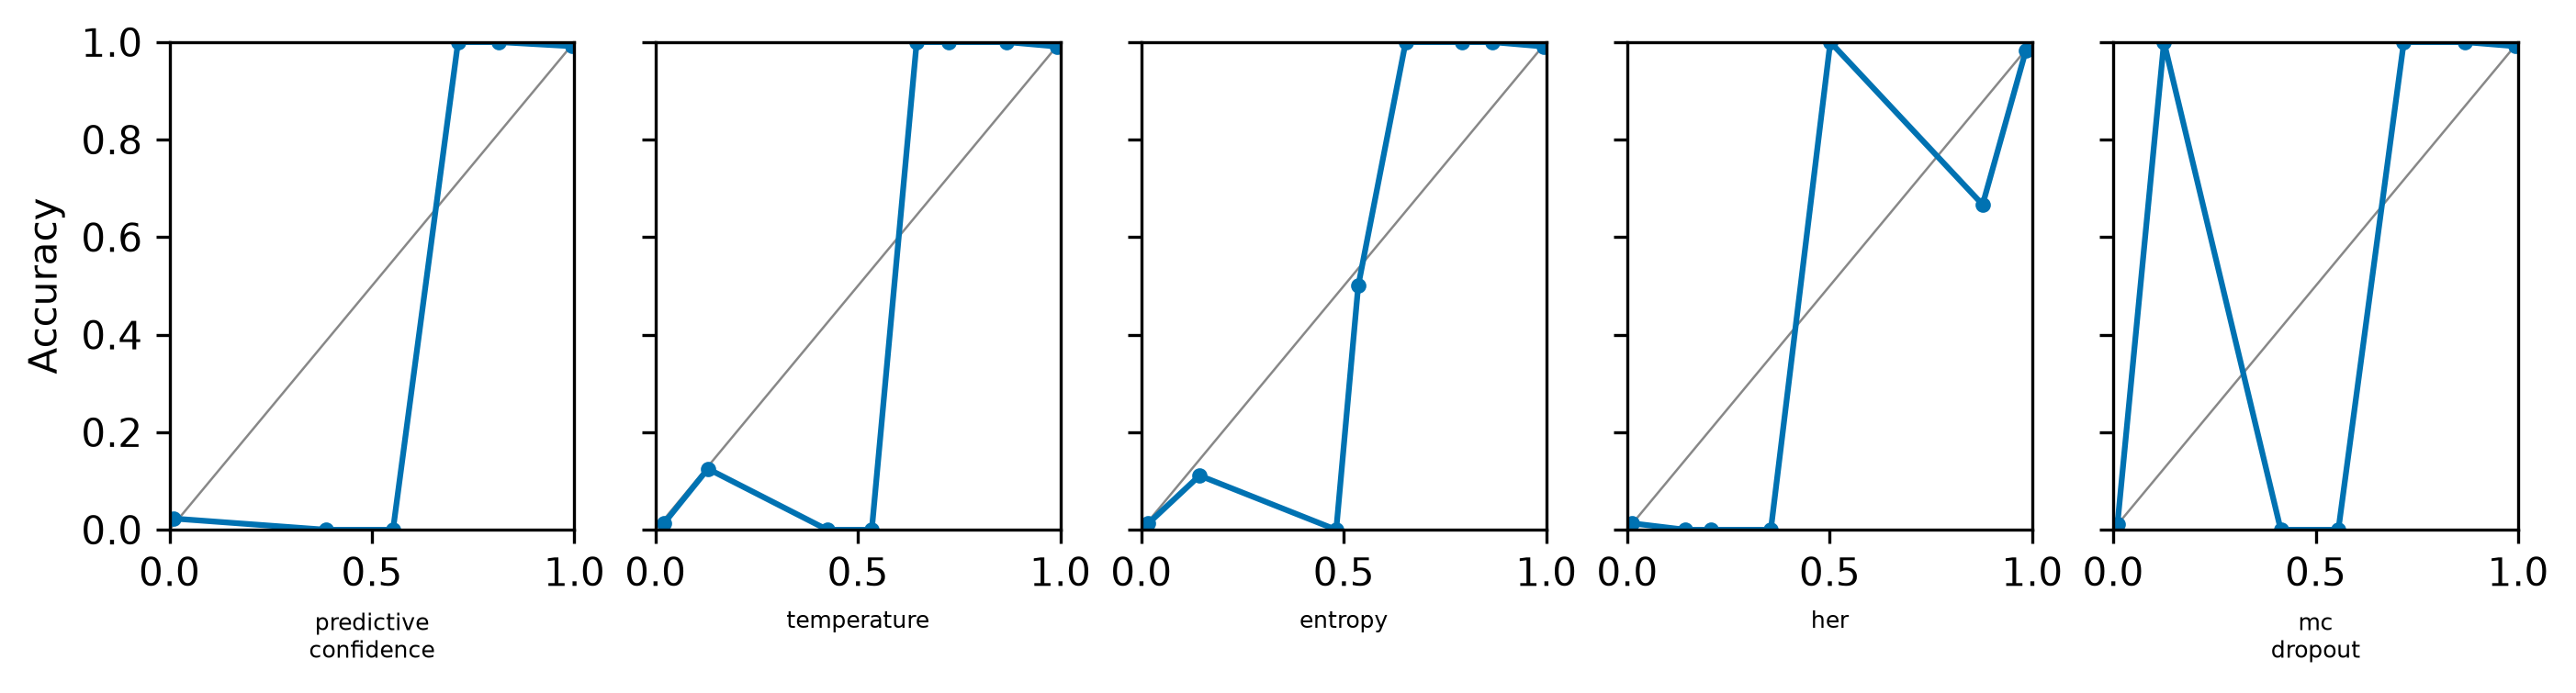
\includegraphics[width=\textwidth]{fig_auth_calibration.png}
  \caption{Reliability diagrams of the authenticator at six views for five confidence estimates (raw predictive confidence, temperature scaling, entropy mapping, HER and MC dropout); calibration maps fitted on the validation split and evaluated on the test split}
  \label{fig:app_calib}
\end{figure}

\subsection{Authentication over Seeds}
\begin{figure}[H]
  \centering
  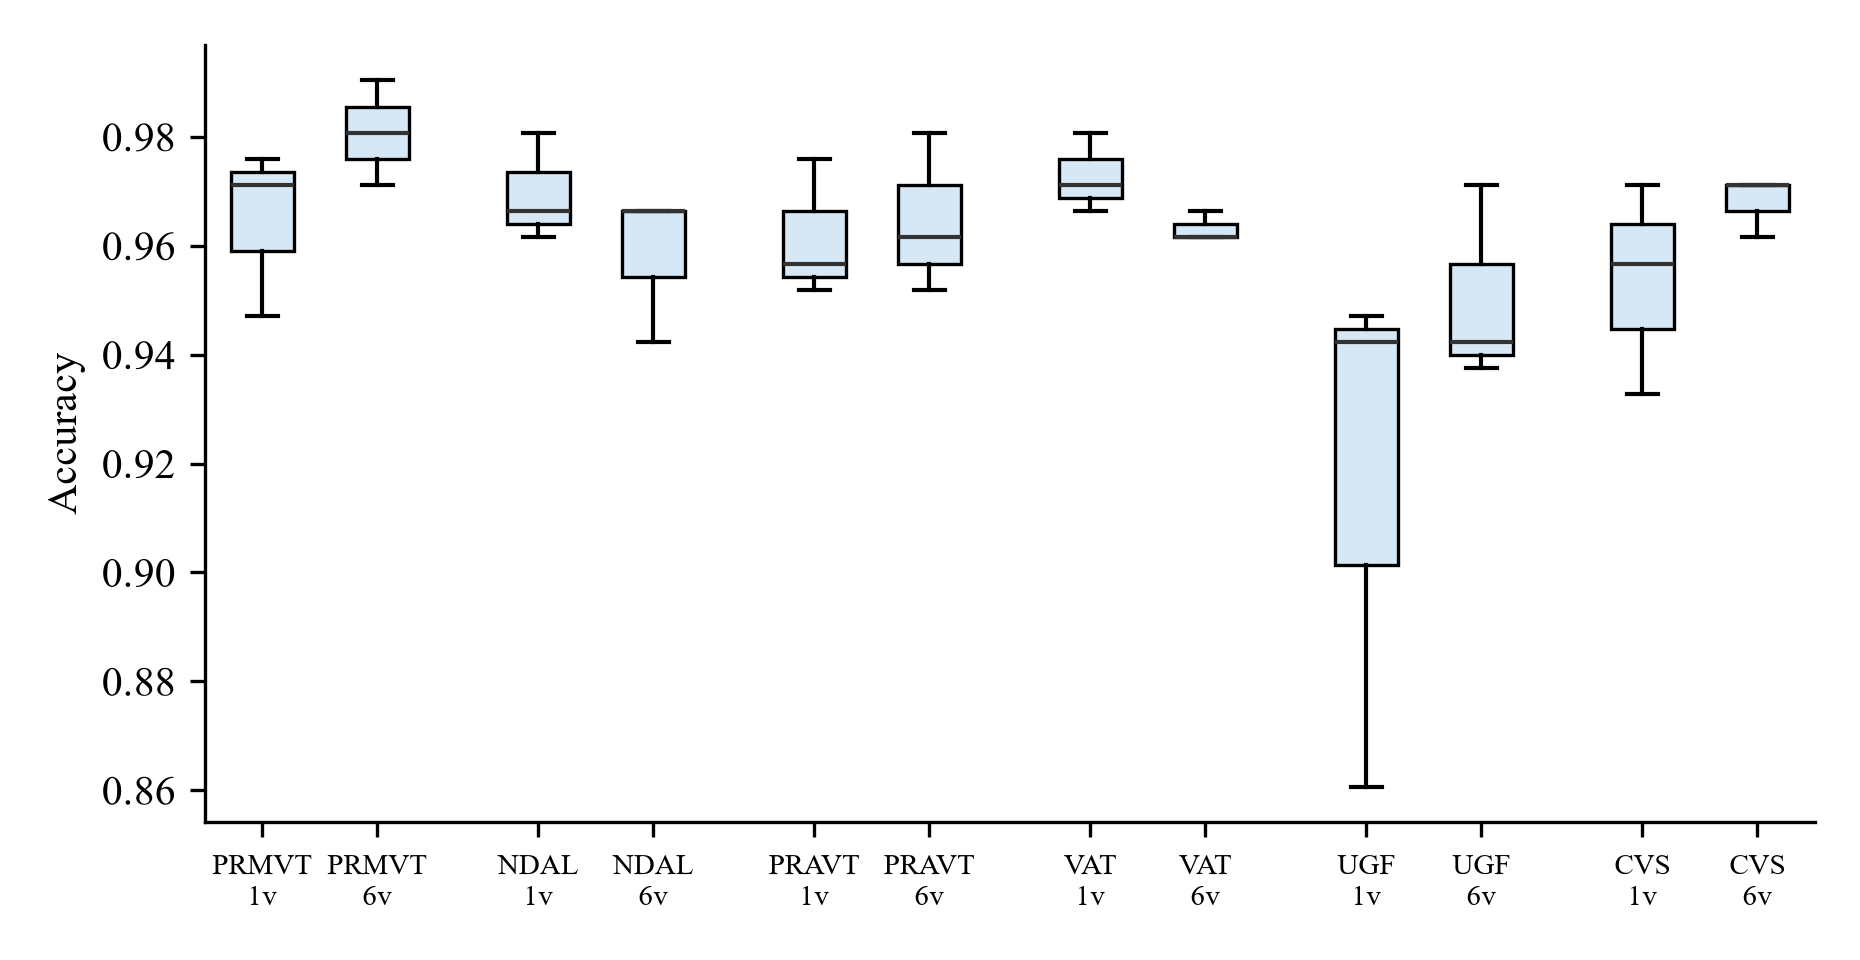
\includegraphics[width=0.8\textwidth]{fig_auth_multiseed.png}
  \caption{Spread of test accuracy over seeds 42, 43 and 44 at one view (1v) and six views (6v) for the main training variants}
  \label{fig:app_multiseed}
\end{figure}

\clearpage
\section{Configuration Parameters}
\label{app:config}

\begin{table}[H]
\centering
\caption{Main configuration parameters of SARA (\texttt{config.py})}
\label{tab:app_config}
\footnotesize
\begin{tabular}{|L{6.4cm}|C{1.9cm}|L{5.8cm}|}
\hline
\textbf{Setting (name in the code)} & \textbf{Value} & \textbf{What it controls} \\ \hline
OCR\_PIPELINE & v2 & Which text-reading pipeline is used (Section~\ref{sec:ocr_method}) \\ \hline
OCR\_V2\_MIN\_CONF & 0.2 & Words the reader is less sure about than this are dropped \\ \hline
OCR\_CANVAS\_SIZE & 2560 & Picture size used to find text; 640 is faster on the Pi but less accurate \\ \hline
OCR\_V2\_DECODER & greedy & How the reader turns its output into letters (greedy: the best letter at each step) \\ \hline
OCR\_STREAM\_PAGES & on, 4 lines & Pages with at least 4 lines are spoken line by line \\ \hline
CURRENCY\_ANNOUNCE\_CONF & 0.60 & A note is named only when the detector is at least this sure \\ \hline
JAAL\_SAFE\_TAU & 0.99959 & The glass says ``likely genuine'' only above this score; otherwise ``check by hand'' \\ \hline
WATERMARK\_CLEAR\_THRESHOLD & 0.5 & Score above which the watermark counts as present \\ \hline
CAPTURE\_GUIDE\_MIN\_MEAN & 73.87 & A note photo held against light must be at least this bright (0--255) \\ \hline
CAPTURE\_GUIDE\_MIN\_LAPVAR & 106.75 & The photo must be at least this sharp (Laplacian variance) \\ \hline
CAPTURE\_GUIDE\_TIMEOUT\_S & 10 s & If no good photo arrives in this time, the glass asks the user to check by hand \\ \hline
FIELD\_LOG\_SYS\_INTERVAL\_S & 10 s & How often temperature, memory and load are written to the field log \\ \hline
OBJECT\_CONFIDENCE & 0.50 & An object is spoken only when the detector is at least this sure \\ \hline
CURRENCY\_CONFIDENCE & 0.65 & Minimum score of the back-up Taka classifier (MobileNetV3) \\ \hline
OBJECT\_SCAN\_INTERVAL & 1.5 s & How often object mode looks for objects by itself \\ \hline
OBJECT\_ANNOUNCE\_COOLDOWN & 4.0 s & The same object is not repeated within this time \\ \hline
DEFAULT\_VOLUME & 80\% & Loudness when the glass starts \\ \hline
VOLUME\_STEP & 10\% & Loudness change per VOLUME button press \\ \hline
TTS\_QUEUE\_MAXSIZE & 5 & At most this many sentences wait to be spoken \\ \hline
TTS\_INTER\_UTTERANCE\_PAUSE & 0.15 s & Short pause between spoken sentences \\ \hline
ESPEAK\_SPEED / PITCH & 135 wpm / 45 & Speed (words per minute) and pitch of the espeak-ng voice \\ \hline
Button debounce & 250 ms & A second press within this time is ignored (stops accidental double presses) \\ \hline
CAMERA\_WIDTH, CAMERA\_HEIGHT & 640$\times$480 & Picture size taken from the camera \\ \hline
\end{tabular}
\end{table}

\begin{table}[H]
\centering
\caption{Training hyper-parameters of the YOLOv8s Taka detector}
\label{tab:app_yolo}
\small
\begin{tabular}{|L{4.6cm}|L{10.0cm}|}
\hline
\textbf{Setting} & \textbf{Value} \\ \hline
Model & YOLOv8s (11.1 million parameters, 28.5 GFLOPs), starting from weights already trained on COCO \\ \hline
Training rounds (epochs) / stop early if no progress for & 80 / 15 epochs \\ \hline
Picture size / pictures per step (batch) & 640 pixels / 16 \\ \hline
Learning method (optimiser) & SGD; starting learning rate 0.01, final factor 0.01; momentum 0.937; weight decay 0.0005 \\ \hline
Gentle start (warm-up) & 3 epochs \\ \hline
Weights of the three training losses & Box position (CIoU) 7.5; note type (BCE) 0.5; box edges (DFL) 1.5 \\ \hline
Extra random changes during training & Mosaic of four pictures 1.0; mixing two pictures 0.15; colour shift (hue 0.02, saturation 0.7, brightness 0.4); rotation up to 20$^\circ$; shear 5$^\circ$; resize $\pm$50\%; shift 10\% \\ \hline
Mirror flips & Off (left--right and up--down), because a mirrored note is not a real note \\ \hline
Software & Ultralytics 8.4.64, PyTorch 2.6.0 with CUDA 12.4 \\ \hline
\end{tabular}
\end{table}

\section{Reproducing the Results}
\label{app:repro}
\begin{lstlisting}
# Taka detector (Windows, from realtime_bangla_taka_detection/)
python -m venv venv
.\venv\Scripts\pip.exe install -r requirements.txt
.\venv\Scripts\python.exe scripts\download_backgrounds.py
.\venv\Scripts\python.exe scripts\generate_synthetic_dataset.py
.\venv\Scripts\python.exe scripts\train.py
.\venv\Scripts\python.exe scripts\evaluate.py
.\venv\Scripts\python.exe scripts\realtime_detect.py   # live demo

# Smart glass on Raspberry Pi 5 (from savior_glass/)
bash scripts/deploy_pi5.sh                  # packages, environment, models
python scripts/pi5_preflight.py             # check libraries and models
python main.py                              # start the glass
python scripts/benchmark_pi5.py --iters 100 --sustained 30
python scripts/diagnose_glass.py currency   # live frame vs high resolution
python scripts/field_report.py              # summary of the field log

# Smart glass on a laptop with a webcam (preview window, keyboard keys)
SHOW_PREVIEW=1 python main.py
python scripts/run_voice_study.py           # voice questionnaire session
python scripts/run_voice_study.py --results

# OCR benchmark (from savior_glass/ocr_bench/)
python run_task1.py ... run_task6.py        # validation experiments
python run_test.py                          # test set, once per method

# Counterfeit experiments (from realtime_bangla_taka_detection/)
python scripts/eval/jaaltaka_serial_audit.py
python scripts/train/train_watermark_localizer.py 42

# Experiment database
python research_results/results_db.py review
\end{lstlisting}

\section{Spoken Messages}
\label{app:messages}
The glass speaks Bangla. Table~\ref{tab:app_messages} gives the main messages in English translation.

\begin{table}[H]
\centering
\caption{Main spoken messages of SARA (translated from Bangla)}
\label{tab:app_messages}
\begin{tabular}{|L{5.0cm}|L{9.4cm}|}
\hline
\textbf{When} & \textbf{What the glass says} \\ \hline
A note is recognised & ``Five hundred Taka note'' \\ \hline
The counterfeit check is passed & ``Likely genuine'' \\ \hline
The counterfeit check is not passed & ``Check by hand whether it is genuine'' \\ \hline
A note other than 500 or 1,000 Taka (no check available) & ``The counterfeit check was not done'' \\ \hline
The detector is not sure enough & ``Could not confirm the note. Hold it closer.'' \\ \hline
No note is found & ``No note detected. Hold it in front of the camera.'' \\ \hline
The watermark check starts & ``Hold the note up to the light'' \\ \hline
The picture is too dark & ``Hold the note closer to the light'' \\ \hline
The picture is blurred & ``Keep the note still'' \\ \hline
The watermark area cannot be found & ``Hold the note straight in front of the light'' \\ \hline
No good picture within 10 seconds & ``The picture was not clear. Check by hand whether it is genuine.'' \\ \hline
Emotion mode finds a face & ``The person in front looks happy'' \\ \hline
Emotion mode finds no face & ``No face found. Point the camera at a person's face.'' \\ \hline
\end{tabular}
\end{table}

\section{User Study Questionnaire}
\label{app:questions}
The six yes/no questions asked by the voice study tool, translated from Bangla:
\begin{enumerate}[noitemsep]
    \item Was the glass easy to use?
    \item Was the speech of the glass clear?
    \item Did the glass help you recognise banknotes?
    \item Did the glass help you read text?
    \item Can you trust the answers of the glass?
    \item Would you want to use this glass every day?
\end{enumerate}
